%!TEX root = ../../main.tex

\chapter{Image Representation}

\section{Appearance}
\label{sec:appearance}
In the \giraf software-suite there exist various types of images, such as pictograms and profile pictures. Images should be quadratic, have a white background regardless of content and have a black border, as seen in \figref{fig:pictogram_image_view}. 

\todo{Refer to black}

\begin{figure}[!htbp]
    \centering

    \begin{subfigure}[t]{0.4\textwidth}
    	\centering
        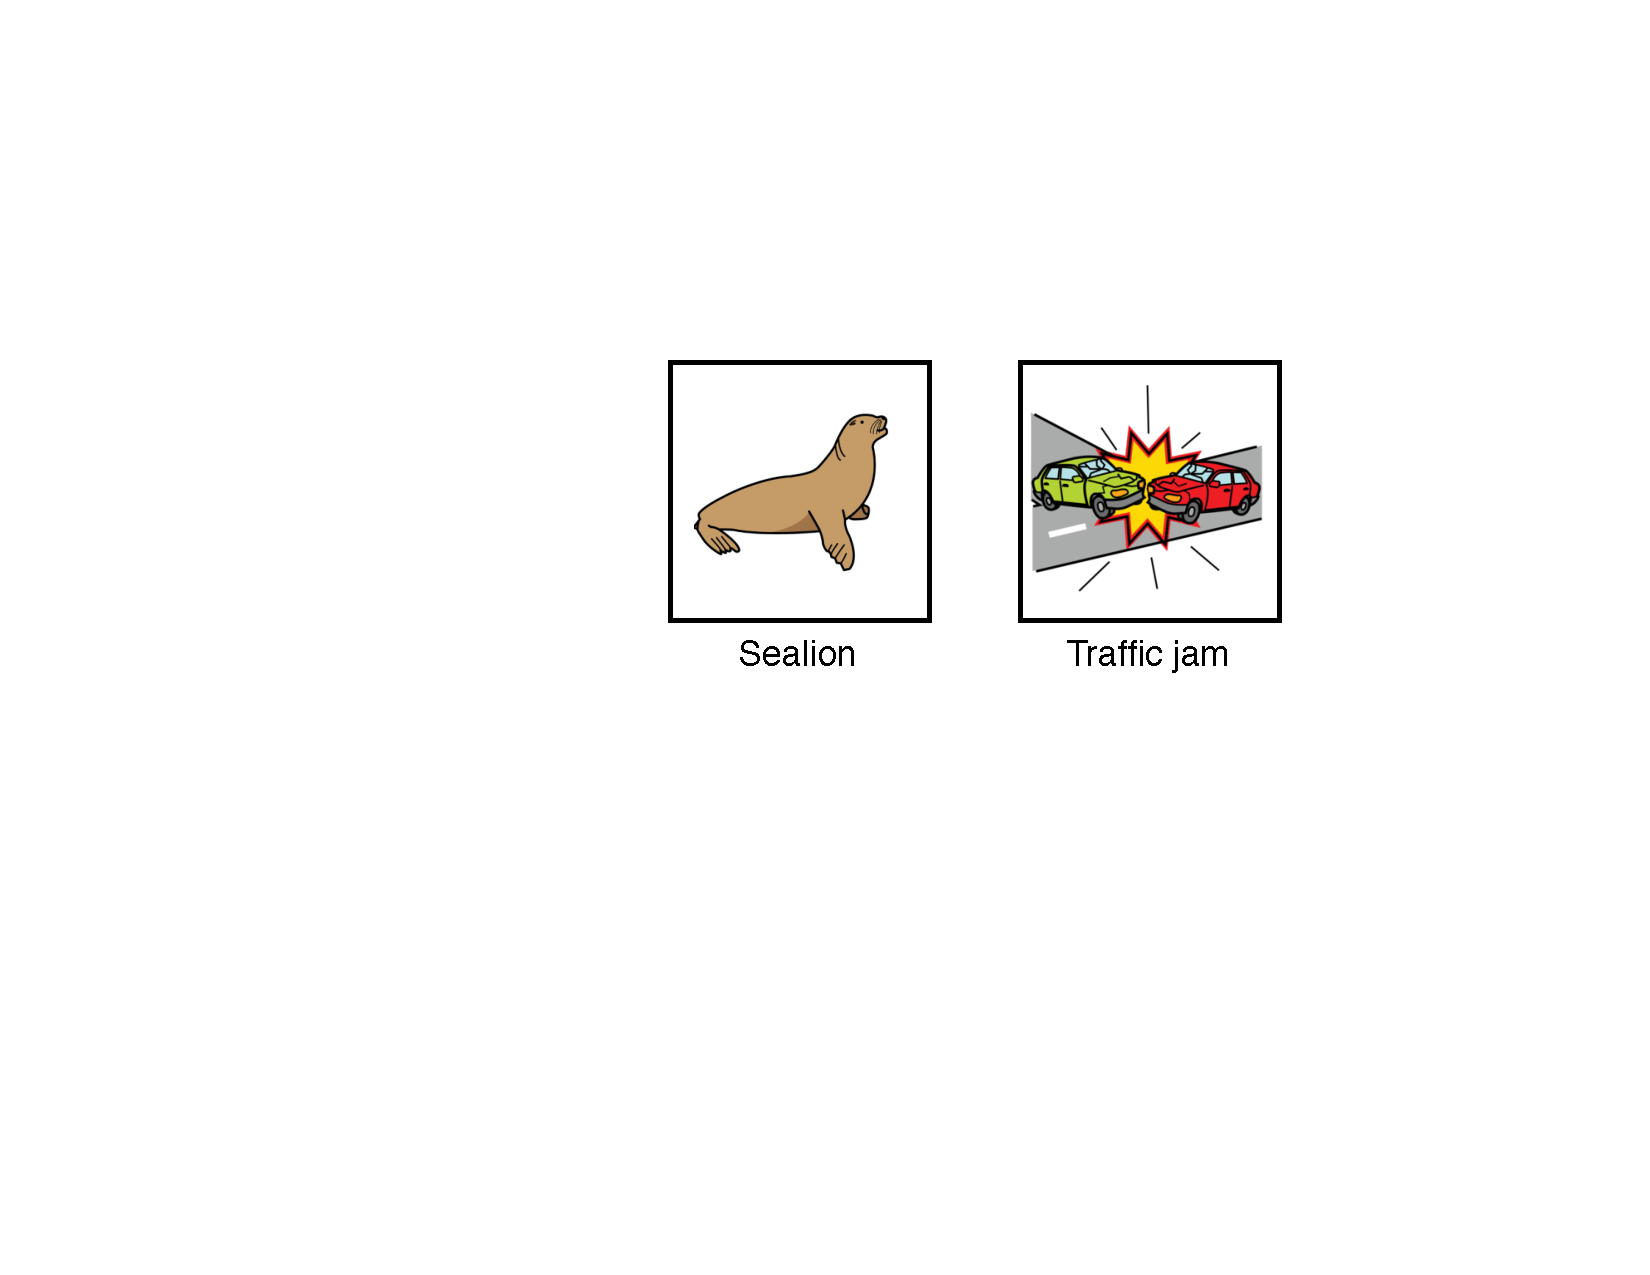
\includegraphics[scale=0.5]{pictogram_image_view_pictograms}
        \caption{Pictograms}
        \label{fig:pictogram_image_view_pictograms}
    \end{subfigure}
    \hspace{5em} 
    \begin{subfigure}[t]{0.4\textwidth}
    	\centering
        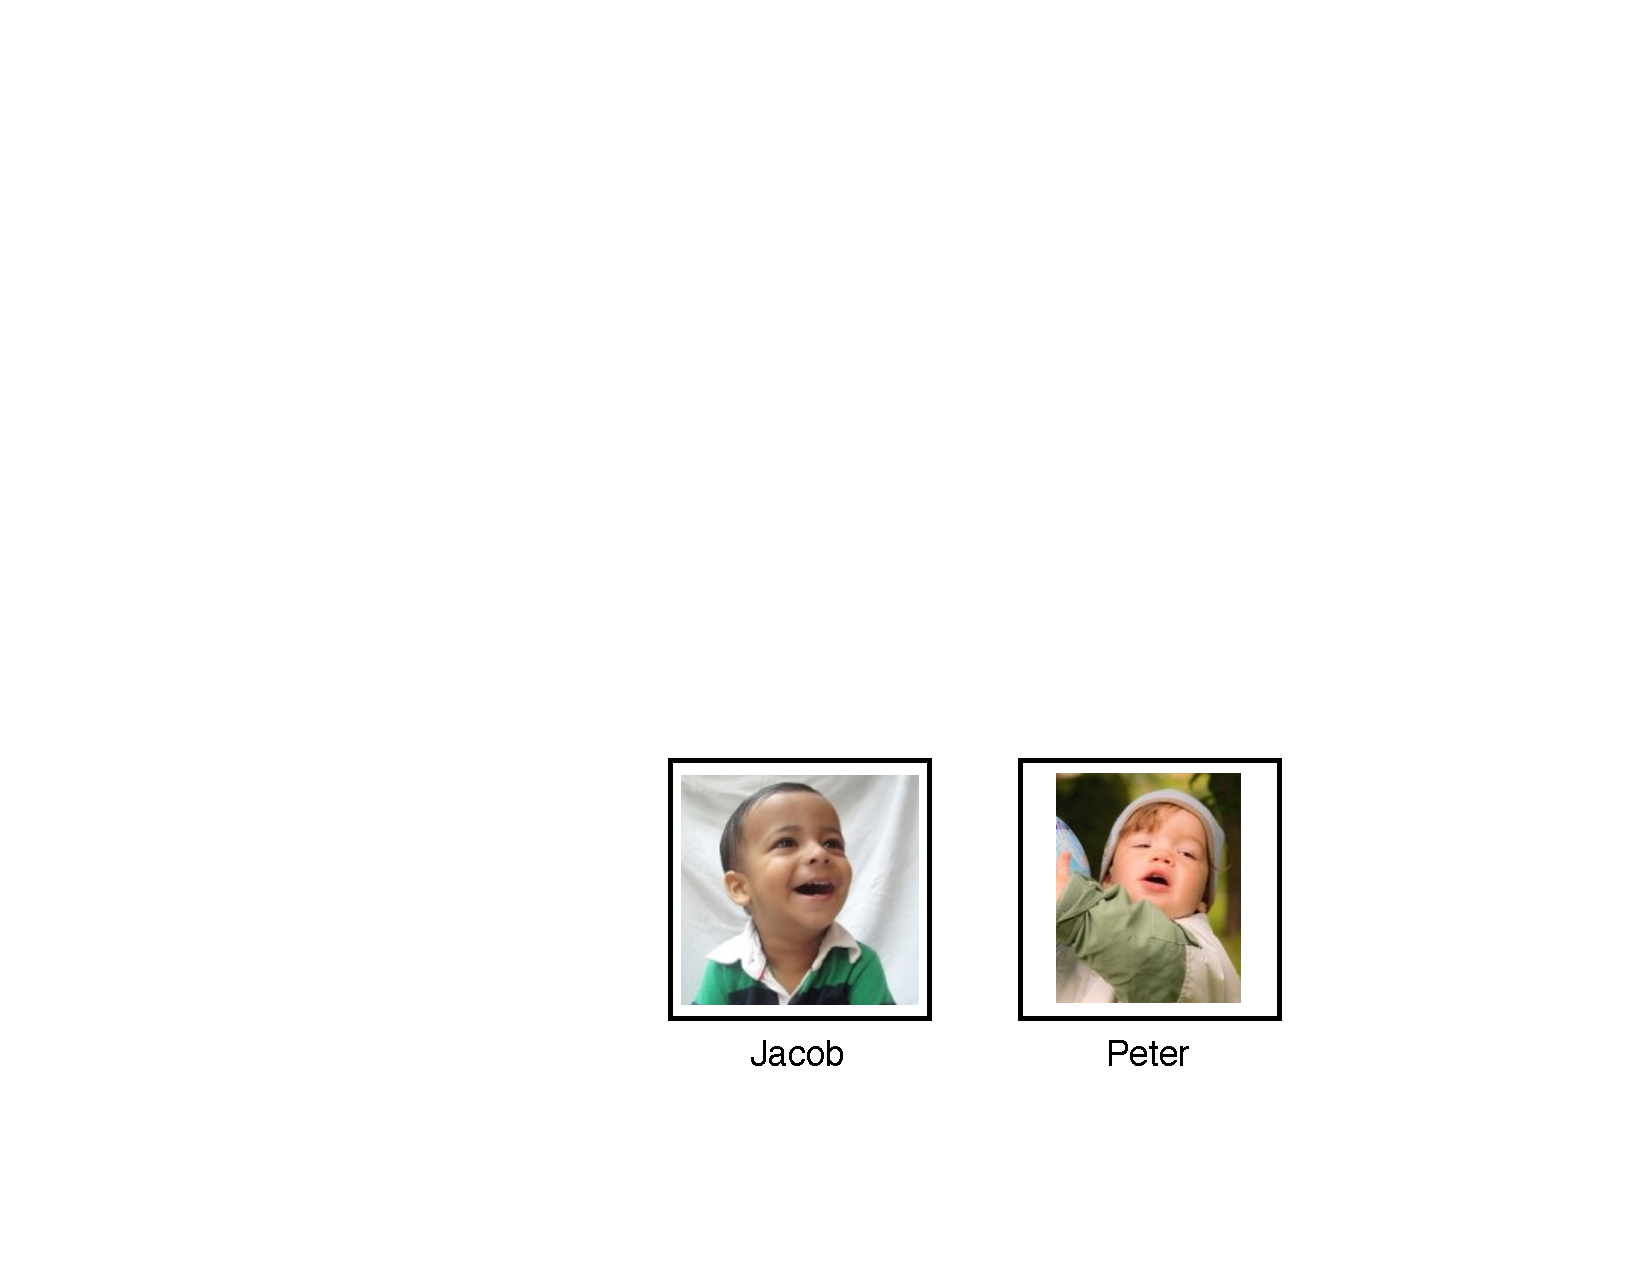
\includegraphics[scale=0.5]{pictogram_image_view_profiles}
        \caption{Profile pictures}
        \label{fig:pictogram_image_view_profiles}
    \end{subfigure}
    
    \caption{Image representation}
    \label{fig:pictogram_image_view}
\end{figure}

\begin{note}
	Profile pictures, as seen in \figref{fig:pictogram_image_view_profiles}, should, as the first profile (Jacob), fit to the canvas. However, many profile pictures are captured in a different way as seen in the second profile (Peter). It is wanted that in the future, when profile pictures are captured, that they only allow for pictures that have the layout of the first profile. For the sake of convenience and backwards compatibility we allow old profile pictures to be as the second.
\end{note}

\noindent
The image view should have a 10 dp padding so that the content gets spacing to the border as seen in \figref{fig:pictograms_padding}.

\begin{figure}[h]
	\centering
	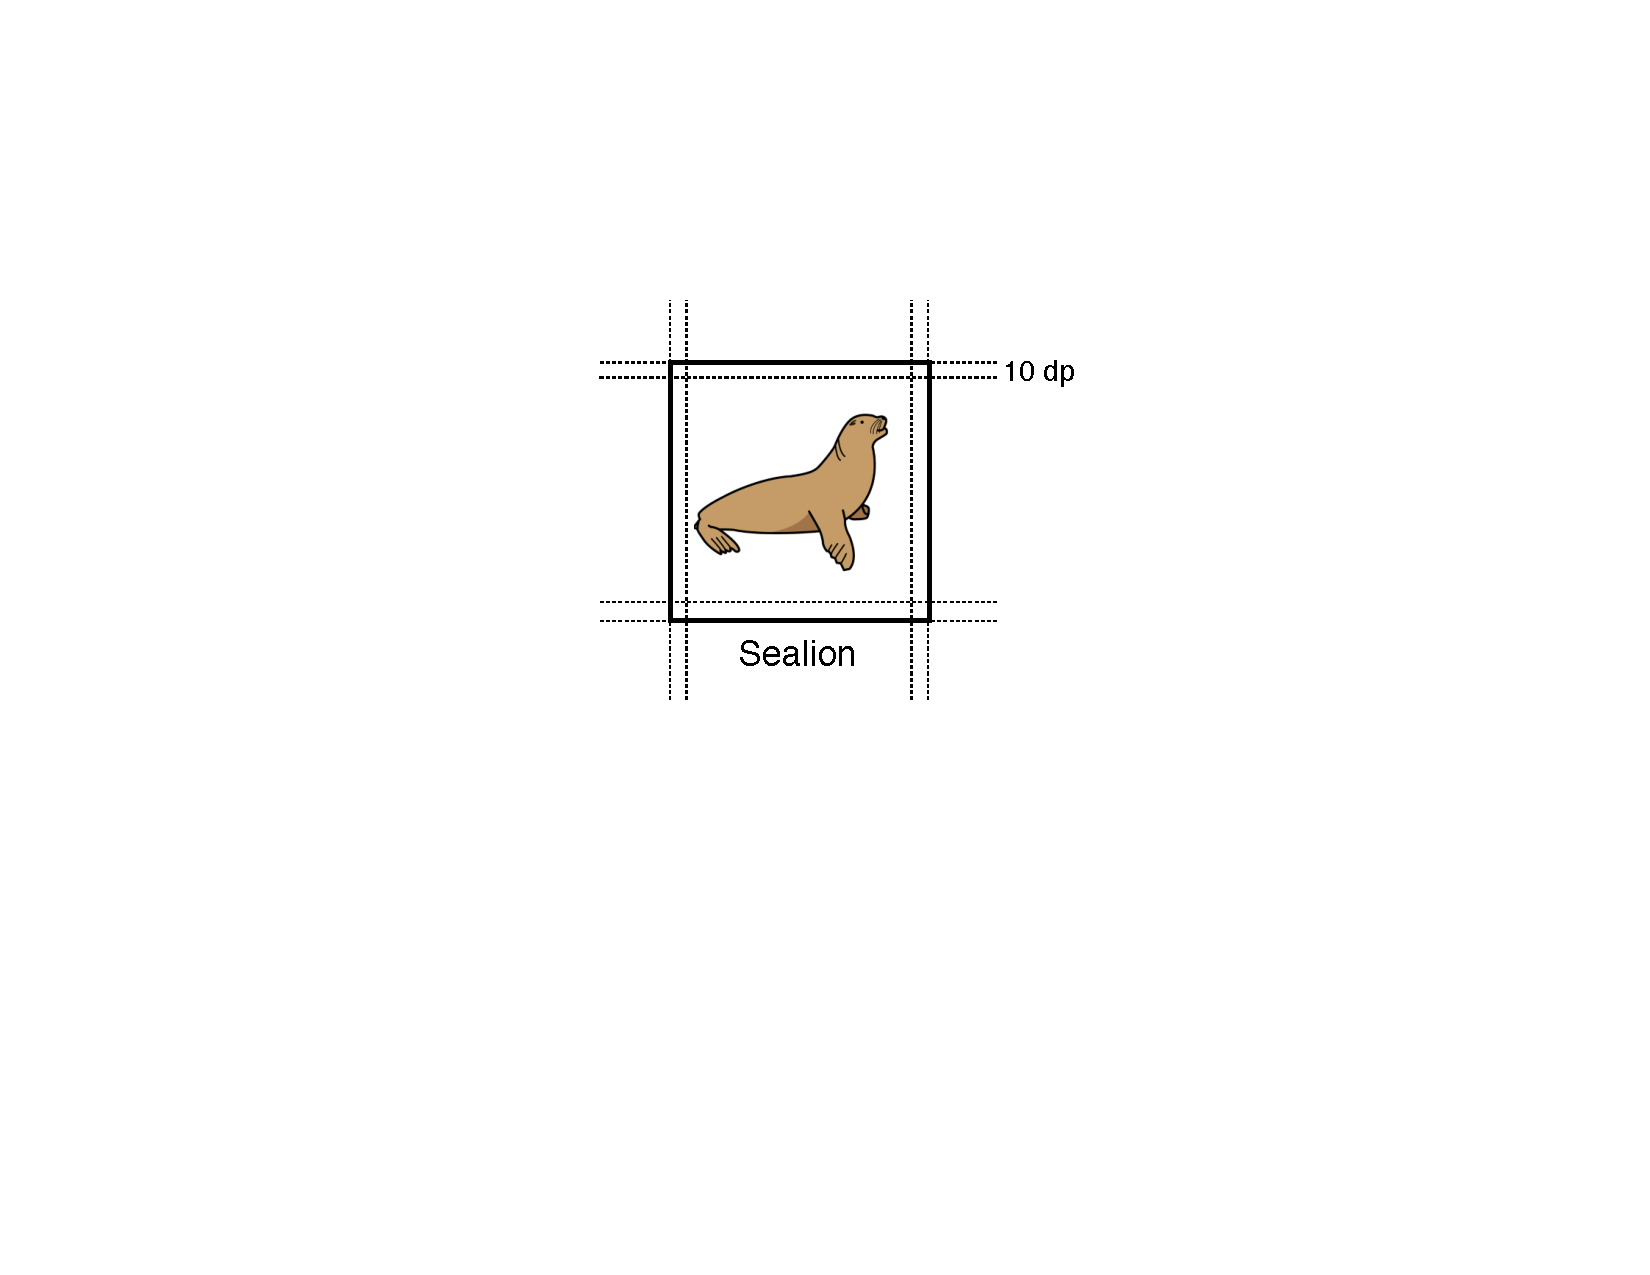
\includegraphics[width=0.35\textwidth]{pictograms_padding}
	\caption{Image representation}
	\label{fig:pictograms_padding}
\end{figure} 
\FloatBarrier

\section{Marking}
\label{sec:marking}
It is often possible to mark images throughout the suite, and whenever this happens one should mark the background of the selected item with an orange color \todo{refer to orange color}, as seen in \figref{fig:pictograms_marked}. 

\begin{figure}[!htbp]
    \centering

    \begin{subfigure}[t]{0.4\textwidth}
    	\centering
        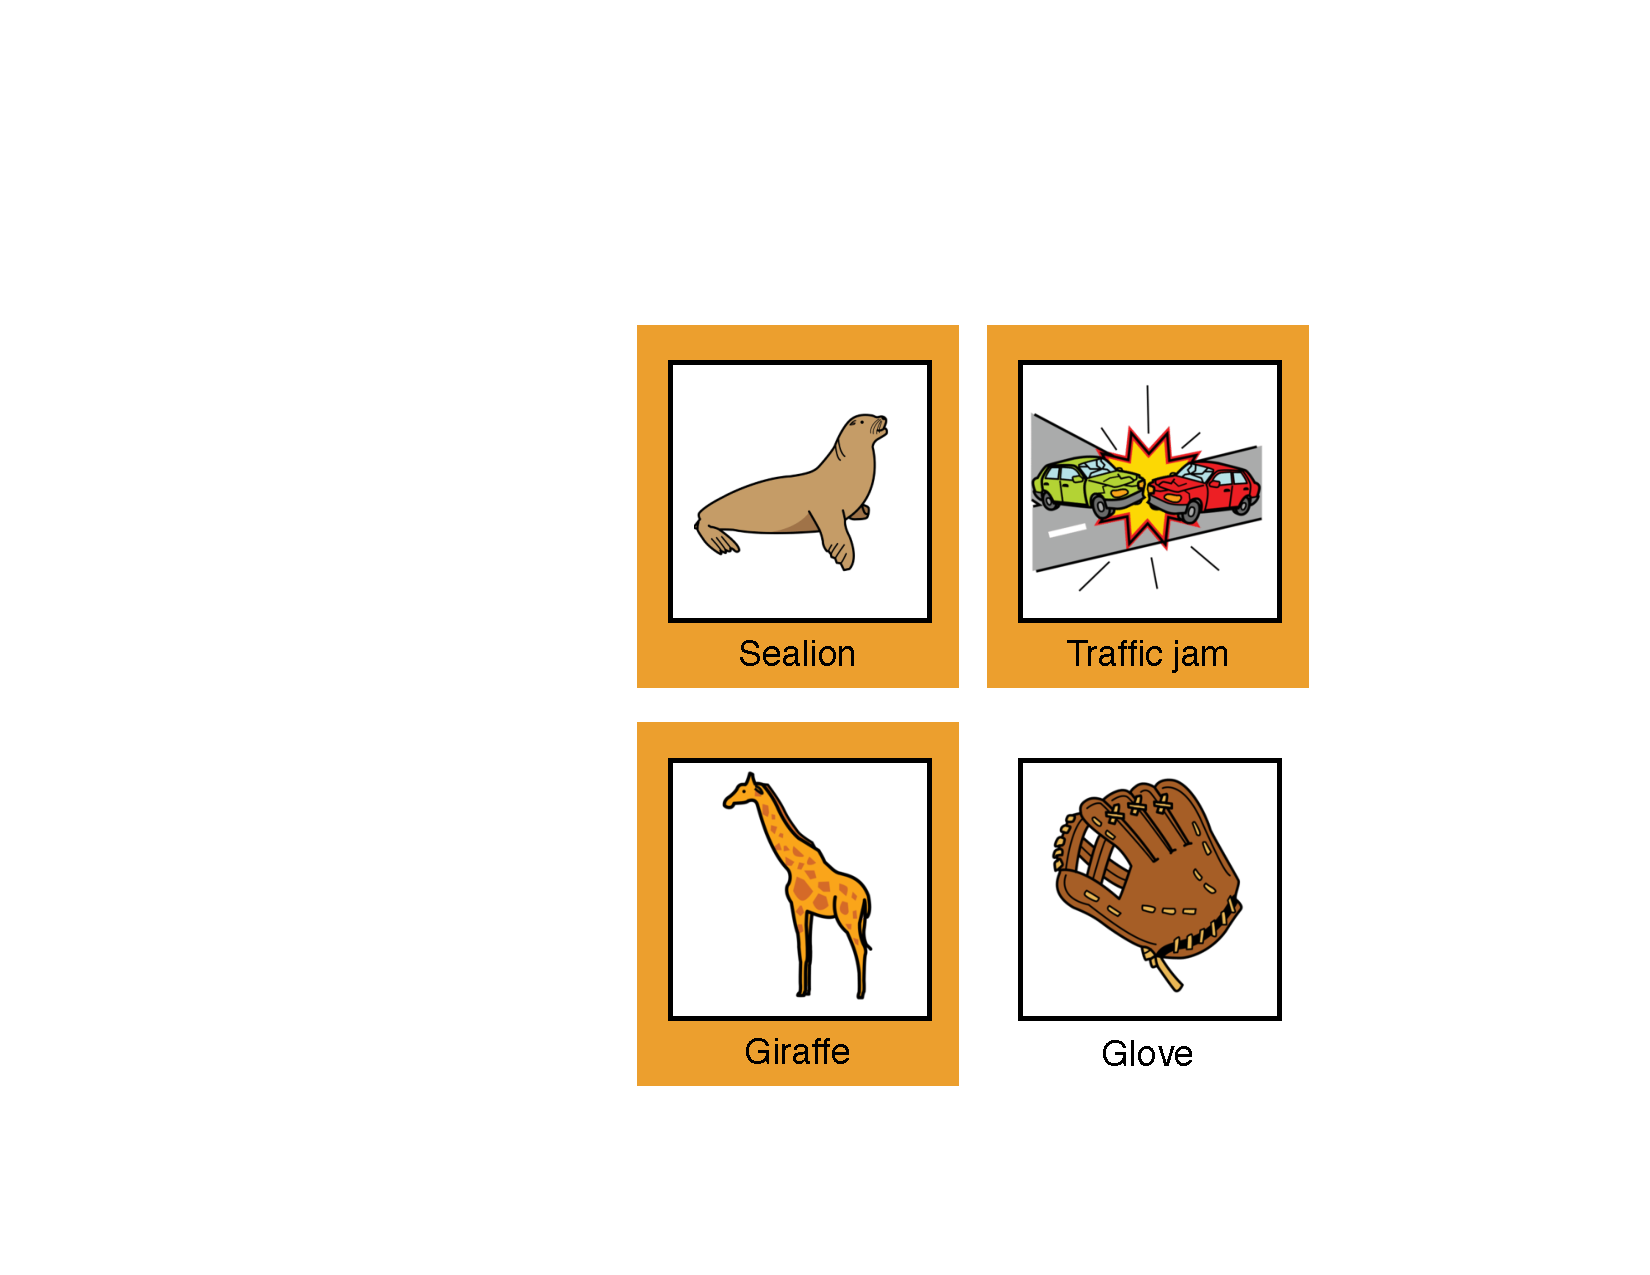
\includegraphics[scale=0.5]{pictograms_marked_correct}
        \caption{Corrected marking}
        \label{fig:pictograms_marked_corect}
    \end{subfigure}
    \hspace{5em} 
    \begin{subfigure}[t]{0.4\textwidth}
    	\centering
        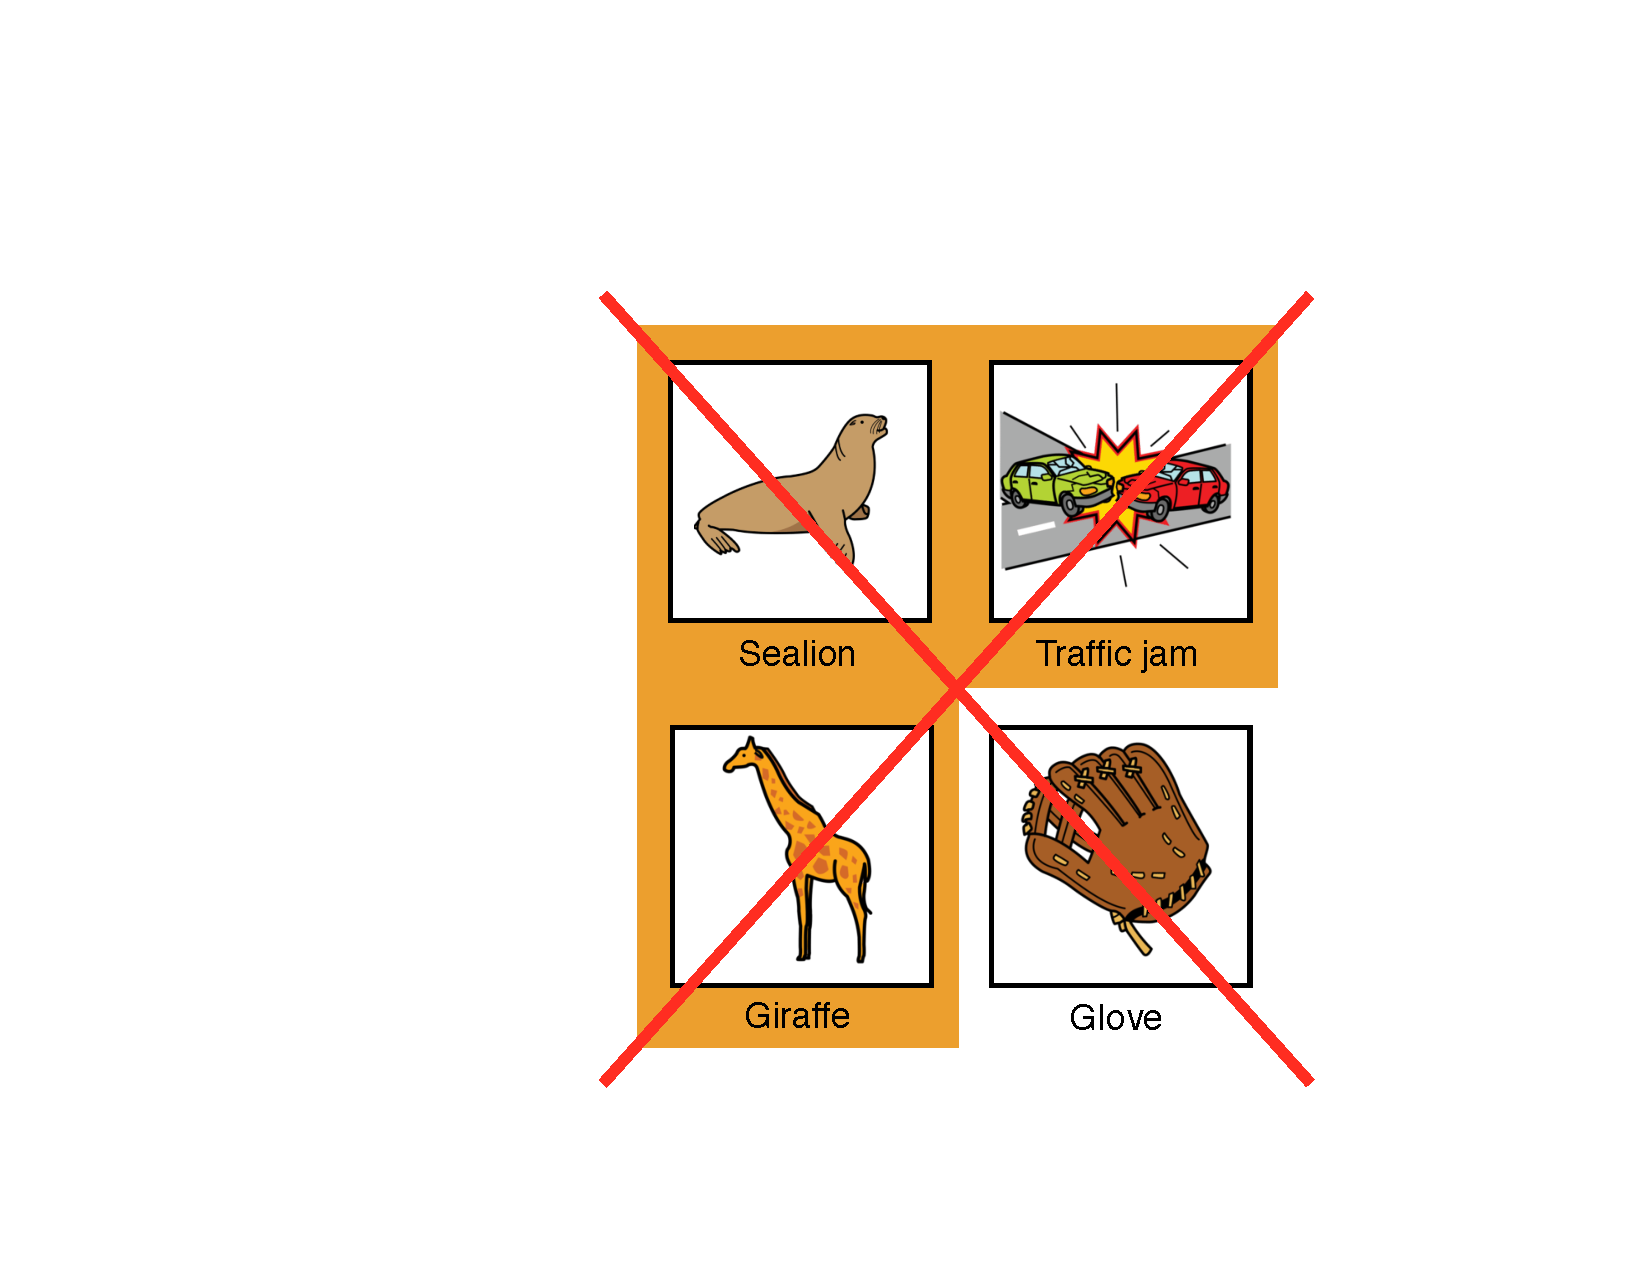
\includegraphics[scale=0.5]{pictograms_marked_wrong}
        \caption{Wrong marking}
        \label{fig:pictograms_marked_wrong}
    \end{subfigure}
    
    \caption{Marking of images}
    \label{fig:pictograms_marked}
\end{figure}

\begin{note}
	It is important that when having multiple marked images that there are some margin between these elements. This should be implemented as seen in \figref{fig:pictograms_marked_corect}, and not as seen in \figref{fig:pictograms_marked_wrong}.
\end{note} 

\section{Indicator overlay}
\label{sec:indicator_overlay}

If one wants to indicate that an image is editable, for instance when picking an icon for a category, the image should have an overlay indicating this as seen in \figref{fig:pictogram_indicator_overlay_editable}. Other types of indicators should look similar, e.g. when indicating that an image is a placeholder for a category it is indicated as seen in \figref{fig:pictogram_indicator_overlay_category}.

\begin{figure}[!htbp]
    \centering

    \begin{subfigure}[t]{0.4\textwidth}
        \centering
        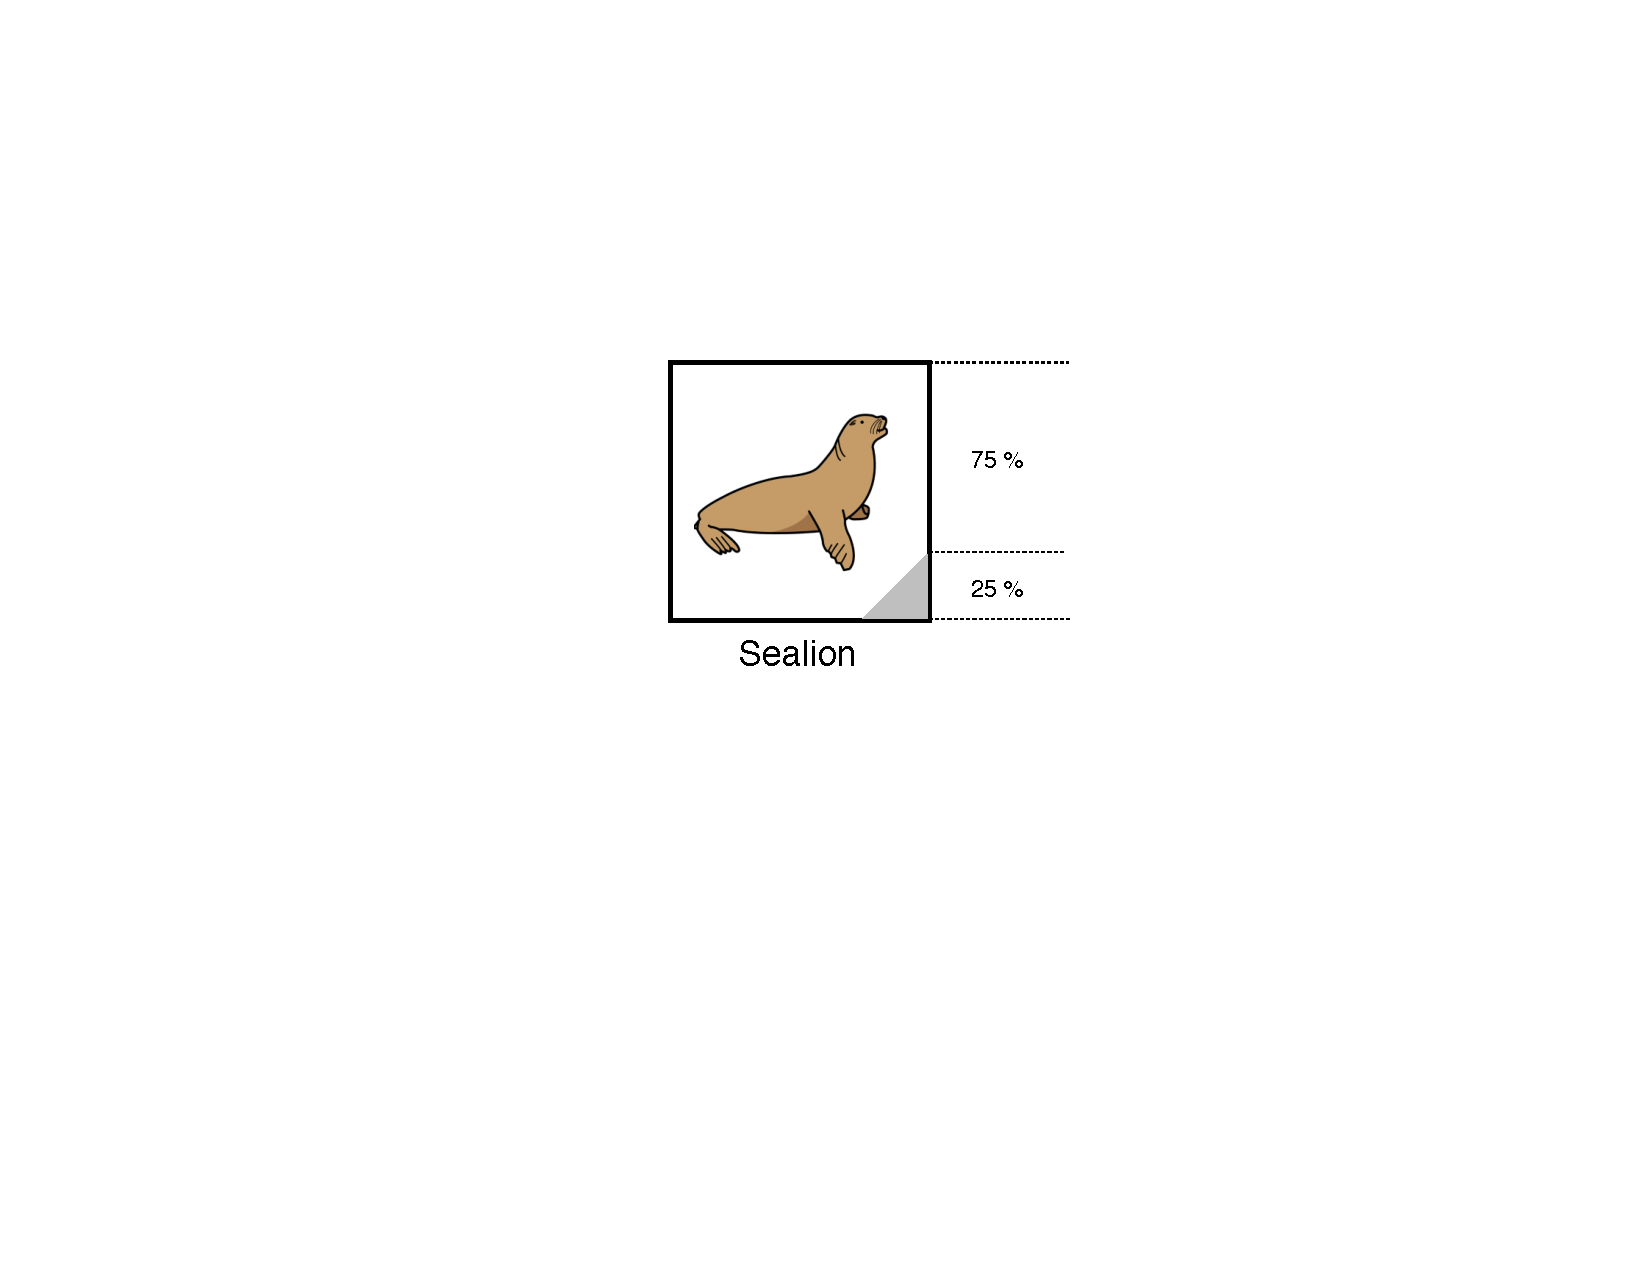
\includegraphics[scale=0.6]{pictogram_indicator_overlay_editable}
        \caption{Editable indicator}
        \label{fig:pictogram_indicator_overlay_editable}
    \end{subfigure}
    \hspace{5em} 
    \begin{subfigure}[t]{0.4\textwidth}
        \centering
        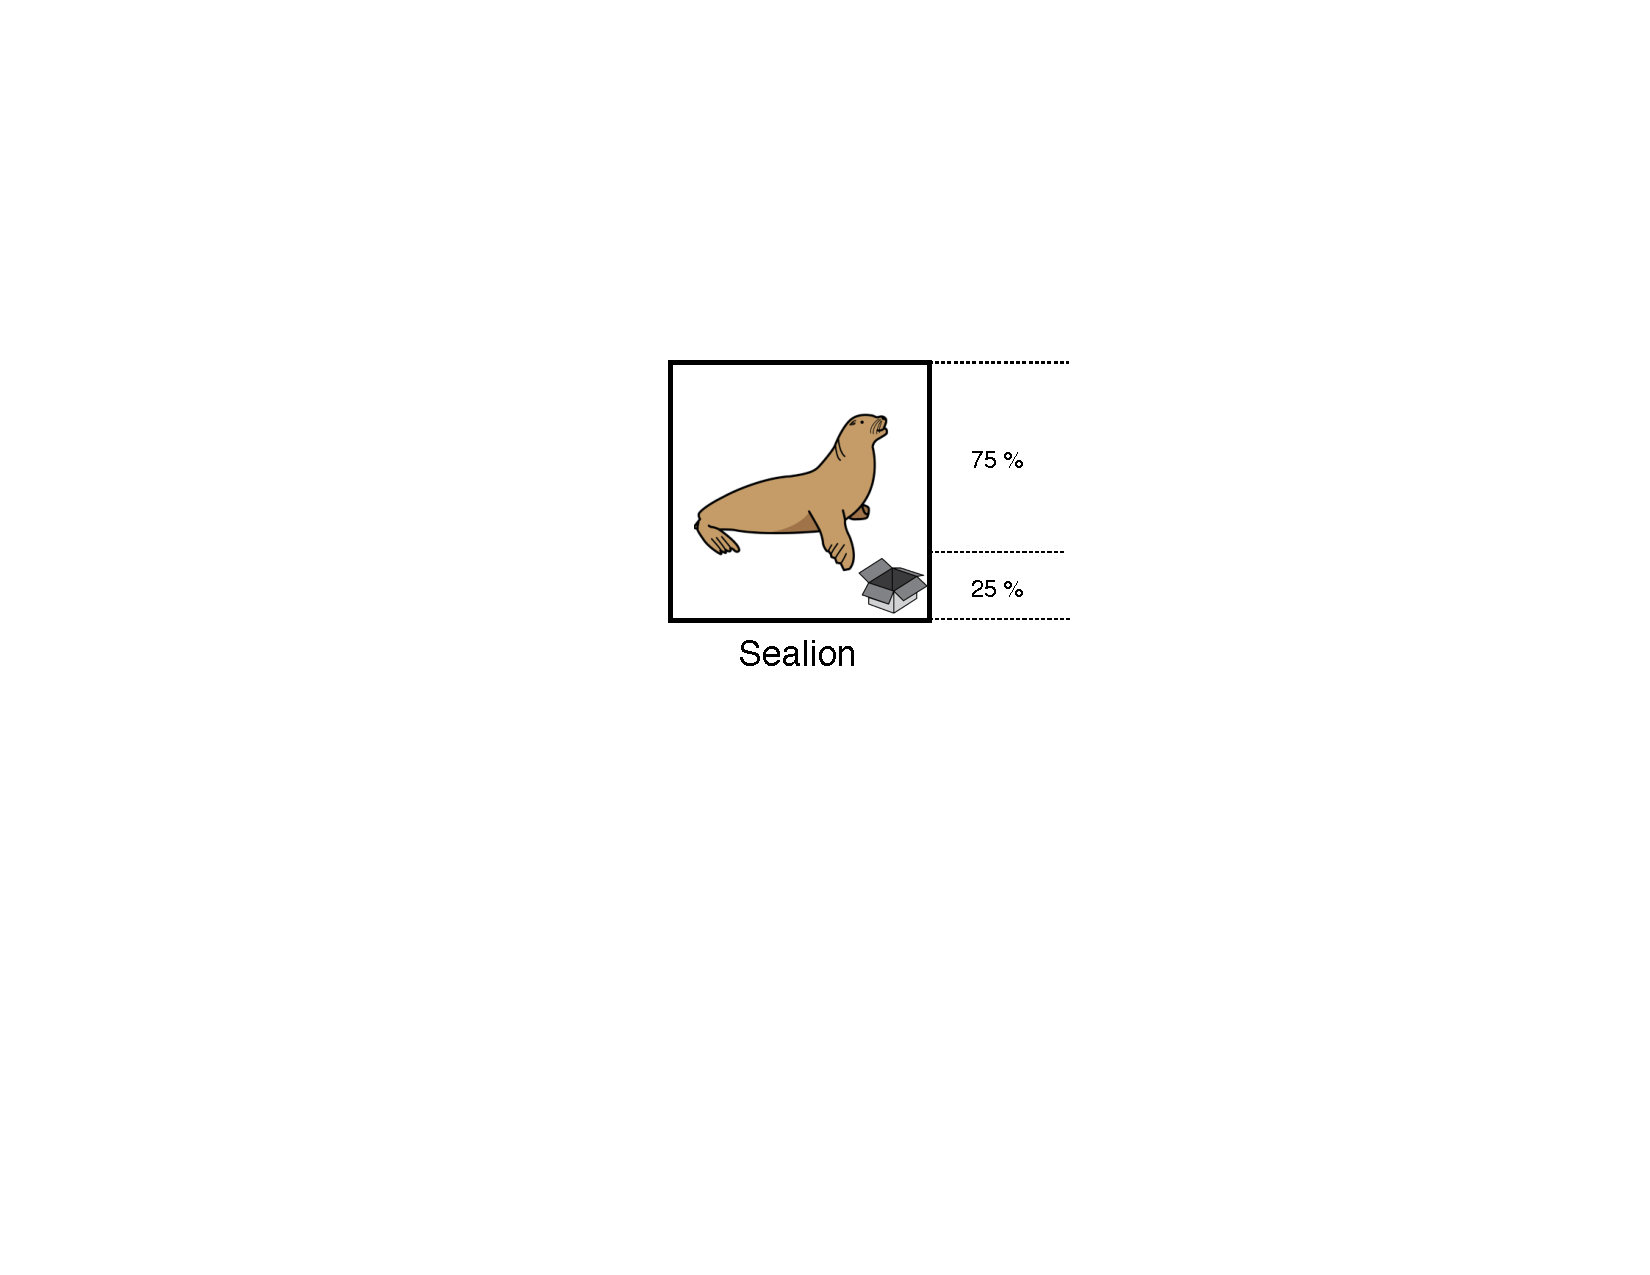
\includegraphics[scale=0.6]{pictogram_indicator_overlay_category}
        \caption{Category indicator}
        \label{fig:pictogram_indicator_overlay_category}
    \end{subfigure}
    
    \caption{Indicator overlays}
    \label{fig:pictograms_marked}
\end{figure}
